\label{Intro.}
Water has been described as being ``at the centre of the planetary drama of the Anthropocene''
\cite{gleesonIlluminatingwatercycle2020}.
It is essential, not only for earth system processes but also in supporting the economic development and continued wellbeing of human societies. Human activities stemming from our reliance on water have profoundly modified the natural water cycle, moving rivers along a trajectory towards a hydrosocial water cycle in which social and power relations dominate the nature of hydrological cycles
\cite{gleesonIlluminatingwatercycle2020,sivapalanSociohydrologynewscience2012,qinTheoreticalframeworkdualistic2014,abbottwatercycleAnthropocene2019,leviaHomogenizationterrestrialwater2020}.
Facing this major transformation, many of the world’s big river basins (which are hot spots of civilization and economic growth) are urgently in need of new models of water governance for sustainability
\cite{bestAnthropogenicstressesworld2019,falkenmarkUnderstandingwaterresilience2019,dibaldassarreSociohydrologyScientificChallenges2019}.
As an integral part of a proposed earth system governance framework, sustainable water governance requires a deep understanding of the complex relationships between people and water
\cite{dibaldassarreSociohydrologyScientificChallenges2019,biermannNavigatingAnthropoceneImproving2012,steffenemergenceevolutionEarth2020}.

For water resources in populated areas, missing governance means missing sustainability
\cite{undpwatergovernancefacilityWaterGovernanceIssue}.
A first important step in identifying transitions towards a hydrosocial water cycle is to identify the different regimes under which it occurs.
According to the United Nations Development Programme (UNDP), three key dimensions of water use are decided by the water governance regime directly: ``How much water can be used?'' (supply), ``How can different services provided by water be balanced?'' (purpose), and ``How can water be allocated equally and efficiently?'' (allocation)
\cite{undpwatergovernancefacilityWaterGovernanceIssue, mariajacobsonUserguideassessing2013, kjellenWatergovernanceperspective2015}.
A regime is defined as a locally stable state of a system’s structure, function, and dominant controls
\cite{carpenterEarlyWarningsRegime2011}.
Large and persistent changes in key system properties may lead to a loss of local stability, potentially resulting in a regime shift with impacts on system outcomes and widespread cascading effects
\cite{rochaCascadingregimeshifts2018, gregrCascadingsocialecologicalcosts2020}.
Regime shifts are both consequences and signals of substantive changes in water governance, and may lead to new challenges to sustainability.

In addition to being caused by changes in key environmental, economic, social and political variables, regime shifts in water governance can be triggered through changes in each of the three key dimensions of governance (supply, purpose, and allocation) %! UNDP year
\cite{undpwatergovernancefacilityWaterGovernanceIssue, mariajacobsonUserguideassessing2013, kjellenWatergovernanceperspective2015}.
First, the supply of water depends not only on climate (with increasing scarcity and unsertainty in many regions) but also on the increasingly insatiable demands from economic activities such as irrigation and industry; water storage can resolve some but not all of these issues
\cite{greveGlobalassessmentwater2018,wadaHumanwaterinterface2017,qinFlexibilityintensityglobal2019}.
Second, the purposes for which water is used are in need of balanced between consumptive uses (e.g., drinking and food production) and non-consumptive uses (e.g., energy production or urban services)
\cite{liuWaterscarcityassessments2017,florkeWatercompetitioncities2018,kleemannQuantifyinginterregionalflows2020}.
Water governance can be viewed as the process of assigning weights to each of these different purposes and enforcing the resulting rules.
Third, the allocation of water across the whole basin is influenced not only by regional environmental context but also by local socio-economic trends and regions’ comparative economic advantages, which can be altered by changing social and political drivers
\cite{roobavannanRoleSectoralTransformation2017,speedBasinwaterallocation2013}.
Despite the obvious relevance of substantive changes in any of the three dimensions of water governance, the lack of a simple but comprehensive approach to identifying changes in water governance regimes makes it difficult to achieve water governance for sustainability (Figure~\ref{fig:framework}).

As an informative example, we focus on the Yellow River Basin (YRB, see \textit{Appendix} Methods S1 and Figure S1 for details).
With drastically anthropogenic intervention, the YRB experienced the most intense water challenges in China, leading to long-standing sustainability barriers.
% 半个世纪前,黄河巨大的泥沙负荷不仅给黄河带来了灾难,也给黄河的用水带来了困难。
From about 550BC until half a century ago, flooding and the huge sediment loads of the Yellow River brought frequent human disasters, and the constant shifts of channels made it difficult for its governance
\cite{wangReducedsedimenttransport2016,liDecadalwaterstorage2020}.
Since the 1960s, the implementation of conservation measures, regulation reservoirs, and levee constructions have contained the issues caused by high-sediment loads
\cite{wangReducedsedimenttransport2016,wuEvolutioneffectssocialecological2020}.
However, water over-use has led to drying up of the Yellow River, creating new governance challenges that have been addressed through a range of related policies (e.g., regulating water use and limiting water withdrawals)
\cite{xiaDevelopmentWaterAllocation2012}.
Today, it is still impossible to completely cover water demands, balance trade-offs between ecosystem services, and lead to equities in different regions; -who gets water, when and how is still an open question for sustainable water governance
\cite{wangYellowRiverwater2019,wohlfartSocialecologicalchallengesYellow2016}.
The YRB has been among the most rapidly-changing large river basins in the world, with myriad responses to the endless governance challenges induced by environmental, economic, social and political factors. Identifying regime shifts in water governance within the YRB can thus provide crucial insights into the world’s rapidly-changing big river basins and the ways in which governance may respond to meeting challenges to their sustainability.

% 这里我们整合了三个方向,提出了描绘流域人水关系的指数
We first use the three key dimensions (supply, purpose and allocation) of water governance to develop an Integrated Water Governance Index (IWGI) that can detect and describe changes in water governance at a basin scale (see Figure~\ref{fig:framework} and methods).
% 使用案例研究
Then, by applying the index to a typical rapid-changing big river basin (the YRB), we show how the index can be used to analyse the complicated regimes of water governance and their main causes in a comprehensive but simple way.
% 最后总结出一般性框架
Finally, we propose a general regime transition scheme as a practical guideline for a coordinated approach to exploring the challenges faced by big river basin governance.

\begin{figure*}%[htbp]
	%! I don't know that fig.1 adds much, the explanatory text to the figure is the key.
	\centering
	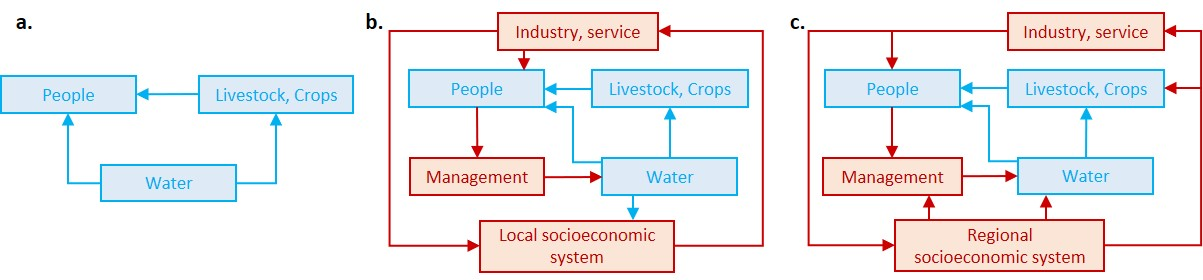
\includegraphics[width=0.9\textwidth]{main/framework.jpg}
	\caption{
		A framework for understanding the relationship between transitional water governance regimes and eventual transformation to a hydrosocial cycle. We aim to detect regime shifts using a simple and comprehensive index.
		% 图A是水资源利用的三个维度。每个维度都有两个极点(红色字表示),指示水资源利用在该轴上的两个变化方向。
		\textbf{A:} there are three key dimensions (supply, purpose and allocation) of water governance (see Methods for details). Each dimension has two poles (denoted in red) which indicate the two potential directions of changes along that axis: (1) ``supply'' shifts between scarcity and abundance. (2) ``purpose'' is weighted between consumptive services or non-consumptive uses. (3) ``allocation'' changes between balanced or lopsided.
		% 图B是将三个维度结合后的变化情况。因上述三个维度随着社会发展而不断变化,其组合的水资源利用状态也不同。这个过程中当突变发生时,可能标志着水资源利用发生了稳态转换,因此我们需要一个指标来监测其变化。
		\textbf{B:} governance changes are an emergent outcome of trends across the three dimensions. Water governance status changes along a trajectory towards a hydrosocial water cycle. When abrupt change occurs, it may indicate a regime shift in water governance
		\cite{steffenTrajectoriesEarthSystem2018,abbottwatercycleAnthropocene2019,leviaHomogenizationterrestrialwater2020}.
	}
	\label{fig:framework}
\end{figure*}
